% !TEX encoding = UTF-8 Unicode
\documentclass[a4paper]{article}

\usepackage[utf8]{inputenc}
\usepackage[slovene,english]{babel}
\usepackage{sty/erk}
\usepackage{graphicx}
\usepackage[autostyle=false]{csquotes}
\usepackage[backend=biber]{biblatex}
\usepackage{times}
\usepackage[top=22.5mm, bottom=22.5mm, left=22.5mm, right=22.5mm]{geometry}

% Slike
\graphicspath{ {./fig/} }
% Literatura
\addbibresource{reference.bib}
% To avoid footnote on cover page:
\def\footnotemark{}



\begin{document}
\begin{sloppypar}
\title{Pregled programirljivih logičnih vezij vgrajenih v C2000 družino
       mikrokrmilnikov}

\author{Andrej Kenda, Mitja Nemec}
% 
\affiliation{Univerza v Ljubljani, Fakulteta za elektrotehniko, Tržaška 25,
             1000 Ljubljana, Slovenija}

\email{E-pošta: andrej@kenda.one}

\maketitle



\begin{abstract}{Povzetek}
FPGA integrated circuits are often indispensable in practice, but their
integration into the system is often demanding and costly. In this article, we
explore one of the answers to this problem offered by the manufacturer Texas
Instruments. In their microcontrollers series C2000, there is an additional
coprocessor, called ``CLB'', which is similar to a FPGA. The article offers an
overview of said coprocessor, its detailed structure, how it is connected to
the rest of the microcontroller and its capabilities.
\end{abstract}

\selectlanguage{slovene}



\section{Uvod}
Pri oblikovanju vdelanih sistemov se zaradi preprostega programiranja in
cenovne ugodnosti najpogosteje poslužujemo mikrokrmilnikov različnih
proizvajalcev. Na začetku oblikovalnega procesa, v včasih preveliki ponudbi,
izberemo čip, ki najbolje ustreza našim zahtevam.

Obstajajo pa tudi aplikacije, ki jim konvencionalni mikrokrmilniki niso kos. Tu
nastopi iskanje drugačnih rešitev. Če imamo srečo, morda odkrijemo kakšen ASIC
(angl. application specific integrated circuit), ki ustreza našim potrebam,
vendar je na določenih področjih teh dokaj malo. V določenih aplikacijah nam ne
preostane drugega kot uporaba FPGA (angl. field-programable gate array) vezja.
Ti nam omogočajo postavitev sistema na nizkem nivoju, ki ga lahko prikrojimo
natanko našim zahtevam. FPGA v veliko aplikacijah namestimo poleg prej
omenjenega mikrokrmilnika in ga uporabimo kot dodaten procesor
\cite{chen-fpga-automation}.

Kljub temu, da so FPGA čipi precej zmogljivi, pa je njihova integracija v
sistem težka.  Kadra, ki ima globoko znanje takšnih sistemov je zaradi
zahtevnosti precej malo. FPGA vezja namreč pogosto zahtevajo uporabo zunanjih
RAM in FLASH vezij ter ADC in/ali DAC pretvornikov. Tako že načrtovanje
tiskanega vezja okoli FPGA vezja zahteva več truda, dodaten trud pa zahteva
tudi komunikacija med posameznimi moduli. V kolikor pa je poleg poleg FPGA
prisoten tudi mikrokrmilnik je tak sistem v primerjavi s sistemom, ki temelji
samo na mikrokrmilniku dražji tako za načrtovanje, razvoj programske
opreme kot tudi za izdelavo. Proizvajalci FPGA vezij na te probleme odgovarjajo
z vgradnjo mikrkrmilnika v samo FPGA vezje \cite{fpga-developers-guide}.

Z druge strani na naštete težave odgovarja proizvajalec Texas Instruments s
koprocesorjem CLB (angl. configurable logic block), ki je vdelan v nekaj
njihovih mikrokrmilnikov. Ta naj bi po proizvajalčevih trditvah tako nadomestil
dodaten FPGA, kot tudi omogočil programiranje s preprostim vmesnikom (in s tem
razvijalcu prihranil marsikatero uro) \cite{clb-intro}.


\section{Predstavitev CLB}\label{sec:predstavitev}
CLB koprocesor, ki je del mikrokrmilnika F28379D, proizvajalca Texas
Instruments je sestavljen iz štirih med seboj enakih podsklopov (angl. Tile).
Vsak podsklop je sestavljen iz procesorja (angl. CELL) ter vmesnika za
``priklop'' signalov iz matične naprave (angl. CPU I/F).

Ti signali lahko izvirajo iz različnih perifernih naprav, kot so eCAP, ePWM,
GPIO... iz CLB-ja pa lahko v prav te periferne naprave tudi ``pripeljemo''
izhodni signal, kot njihov vhod.

Interakcija pa ni omejena le z dodatnimi napravami in matičnim procesorjem,
temveč je mogoča tudi med različnimi podsklopi CLB-ja. Možno pa je tudi
proženje prekinitev, na katere lahko procesor ustrezno reagira.

\section{Zgradba CLB modulov}\label{sec:zgradbaclb}
V poglavju \ref{sec:predstavitev} je omeneno, da je sam CLB sestavljen iz
štirih podsklopov. Na sliki \ref{fig:clb_moduli} je videti, da vsak podsklop
vsebuje \cite[Pogl.~26.4]{mcu-ref-manual}:
\begin{itemize}
    \item 3 štirivhodne LUT4 (angl. 4-input lookup table),
    \item 8 trivhodnih izhodnih LUT3 (angl. 3-input lookup table),
    \item 3 števce,
    \item 3 avtomate stanj FSM (angl. finite state machine),
    \item 1 HLC (angl. high level controller) in
    \item 1 nastavljiv preklopni blok.
\end{itemize}

\begin{figure*}[t]
    \begin{center}
        \begin{minipage}[t]{12cm}
            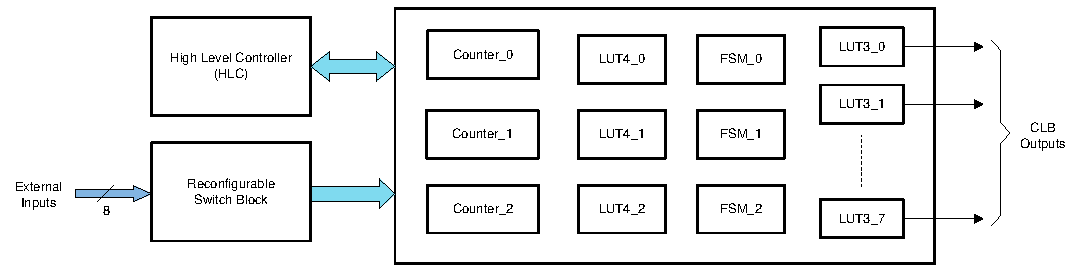
\includegraphics[width=12cm]{clb_moduli}
            \caption{Shematski prikaz modulov na podsklopu CLB koprocesorja
                     \cite[Pogl.~2.3.3]{fpga-to-clb}}
            \label{fig:clb_moduli}
        \end{minipage}
    \end{center}
\end{figure*}

\subsection{LUT moduli}\label{sec:lut}
``LUT4'' modul preslika kombinacijo vhodnih signalov v en izhodni signal na
podlagi prireditvene tabele (slika \ref{fig:lut4} - ``IN0''-``IN3''). Tako
lahko implementiramo poljubno kombinacijo logičnih operacij nad vhodnimi
signali. Preslikava pa se zapiše preko orodja ``CLB Tool'' samo z logičnimi
operacijami ``AND'', ``OR'', ``NOT'' in
``XOR''\cite[Pogl.~3.3]{clb-user-guide}. 

\begin{figure}[htb]
    \centerline{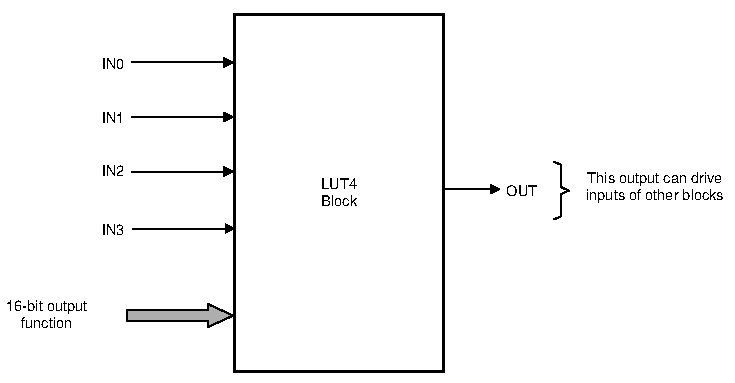
\includegraphics[width=8cm]{shema_lut}}
    \caption{Shematski prikaz štirivhodnega LUT4 modula CLB koprocesorja
             \cite[Pogl.~26.4.4]{mcu-ref-manual}}
    \label{fig:lut4} 
\end{figure} 

``LUT3'' modul je enak ``LUT4'' modulu, le da ima tri namesto štirih vhodov,
ter njegov izhod predstavlja izhod podsklopa (``tile'')
\cite[Pogl.~26.4.4-26.4.5]{mcu-ref-manual}.

\subsection{Števci}
Števec je precej kompleksen modul v CLB-ju, ki omogoča več različnih načinov
delovanja.  Lako deluje kot števec/komparator, samo ko komparator, ki primerja
dve 32-bitni števili, ali pa kot aritmetična enota, ki prišteva oz. odšteva dve
števili ali pa nad enim številom izvede opreacijo dvojiškega premika v levo oz.
desno. S slike \ref{fig:stevec} je moč razbrati štiri funkcijske vhode;
``RESET'', ``MODE 0'', ``MODE 1'' in ``EVENT''. ``RESET'' ob visoki vrednosti
števec postavi na vrednost 0, ``MODE 0'' ob visoki vrednosti omogoči štetje,
``MODE 1'' nastavi smer štetja (visoko - navzgor, nizko - navzdol), signal
``EVENT'' pa ob pozitivnem robu sproži dogodek, na katerega ta odreagira z
nastavljeno računsko operacijo, katere parametre nastavimo z drugima signaloma
(slika \ref{fig:stevec} - ``Static controls'' in ``LOAD VALUE''). Do vsebine
števca lahko dostopamo preko HLC modula (pogl. \ref{sec:hlc}), kjer je ta
označena z zaporedno številko števca (npr. števec 1 - C1).

\begin{figure}[htb]
    \centerline{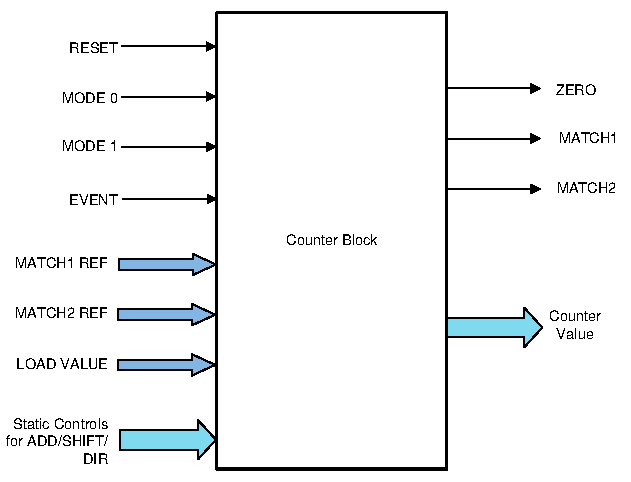
\includegraphics[width=8cm]{shema_stevec}}
    \caption{Shematski prikaz števca CLB koprocesorja
             \cite[Pogl.~26.4.2.1]{mcu-ref-manual}}
    \label{fig:stevec} 
\end{figure} 

Kot izhod iz števca lahko spremljamo signale ``ZERO'', ``MATCH1'' in
``MATCH2''. Prvi prevzame visoko vrednost kadar je vrednost števca 0, ostala
dva pa se vklopita, kadar je vrednost števca enaka nastavljeni pripadajoči
vrednosti. Ko števec doseže svojo maksimalno vrednost ($2^{32}$) ta ``prelije''
in začne šteti od 0.
\cite[Pogl.~26.4.2]{mcu-ref-manual}.

\subsection{FSM moduli}
FSM modul omogoča implementacijo avtomata stanj, ki ima do štiri različna
stanja zakodirana s signali ``S0'' in ``S1''. Avtomat je implementiran z dvema
LUT blokoma: ``S0 Next State LUT'' in ``S1 Next State LUT'' (slika
\ref{fig:fsm}), ki sta po zgradbi povsem enake opisanim v poglavju
\ref{sec:lut}. Ta služita interni modulaciji signalov in operirata z zunanjima
signaloma ``EXT\_IN0'', ``EXT\_IN1'' in vhodoma ``S0'' in ``S1'', ki prevzameta
prejšnjo vrednost izhoda pripadajoče tabele. Izhod avtomata stanj pa določa
``Output LUT'' tabela.

Če aplikacija ne potrebuje uporabe FSM modula, se lahko poslužimo še vhodov
``EXTRA\_EXT\_IN0'' in ``EXTRA\_EXT\_IN1''. V tem primeru celoten modul deluje
kot štirivhodni LUT modul.

\begin{figure}[htb]
    \centerline{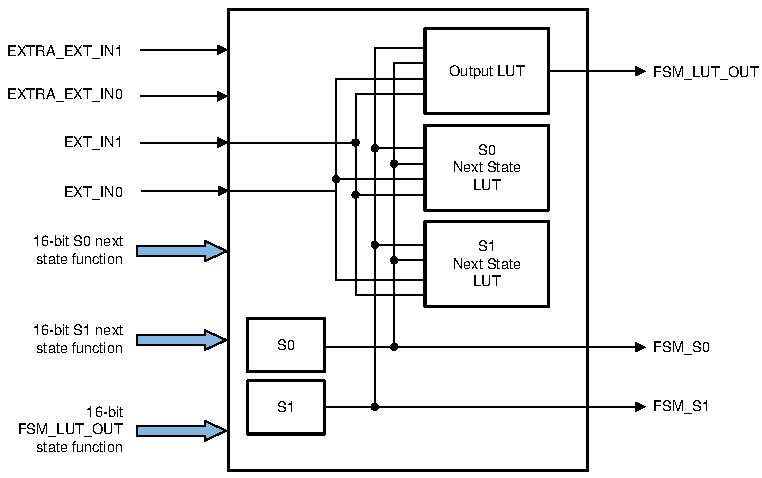
\includegraphics[width=8cm]{shema_fsm}}
    \caption{Shematski prikaz FSM modula CLB koprocesorja
             \cite[Pogl.~26.4.3]{mcu-ref-manual}}
    \label{fig:fsm} 
\end{figure} 

\subsection{HLC modul}\label{sec:hlc}
HLC modul je za razliko od ostale naprave veliko bolj kompleksen (slika
\ref{fig:hlc}).  Gre pravzaprav za zelo okrnjeno procesno jedro, kateremu lahko
sprogramiramo rudimentarno sekvenco ukazov v zbirniku
\cite[Pogl.~26.4.6.2]{mcu-ref-manual}:
\begin{itemize}
    \item ADD/SUB - seštevanje in odštevanje,
    \item MOV/MOV\_T1/MOV\_T2 - premikanje,
    \item PUSH/PULL - pisanje in branje v skupnem spominu,
    \item INTR - proženje prekinitev.
\end{itemize}

To sekvenco pa sprožimo preko zunanjih signalov.

Tako lahko s HLC modulom preko lastnih registrov
``R0''-``R3'' \cite[Pogl.~26.4.6]{mcu-ref-manual} prenašamo podatke med CLB
enoto in glavnim jedrom, kot tudi med trenutno vrednostjo števcev ``C0''-``C2''
in pripadajočimi ``MATCH'' vrednostmi.

\begin{figure}[htb]
    \centerline{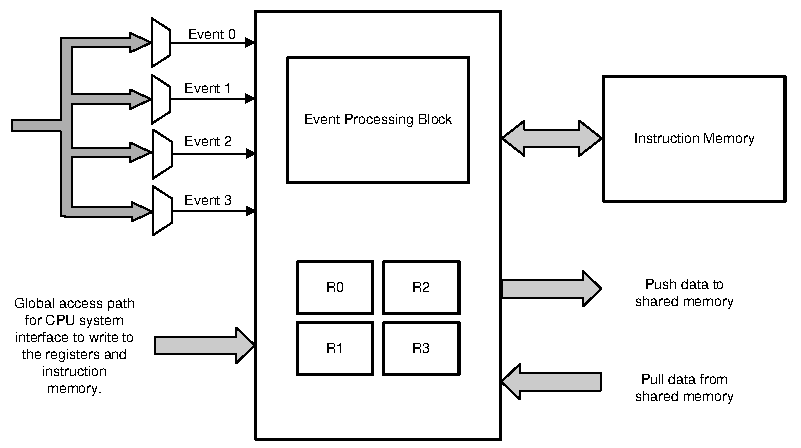
\includegraphics[width=8cm]{shema_hlc}}
    \caption{Shematski prikaz HLC modula CLB koprocesorja
             \cite[Pogl.~26.4.6]{mcu-ref-manual}}
    \label{fig:hlc} 
\end{figure}

\subsection{Preklopni modul}
Ta modul je namenjen izbiri vhodnih signalov, ki lahko izvirajo iz zunanjih
virov, drugih CLB podkslopov (angl. tile) ali pa signal generira modul sam.
Zadnji vir se uporablja le za simulacijske namene. Modul je v orodju ``CLB
Tool'' (Pogl. \ref{sec:clb_tool}) zaradi postavitve predstavljen pod imenom
``BOUNDARY'' \cite[Pogl.~3.3]{clb-user-guide}.


\section{Uporaba CLB}\label{sec:clb_tool}
Za samo programiranje CLB koprocesorja v praksi je proizvajalec Texas
Instruments postavil vmesnik ``CLB Tool'' (slika \ref{fig:clbtool}),
ki nam preko izbire določenih parametrov zgenerira kodo za uporabo v našem
projektu.

\begin{figure}[htb]
    \centerline{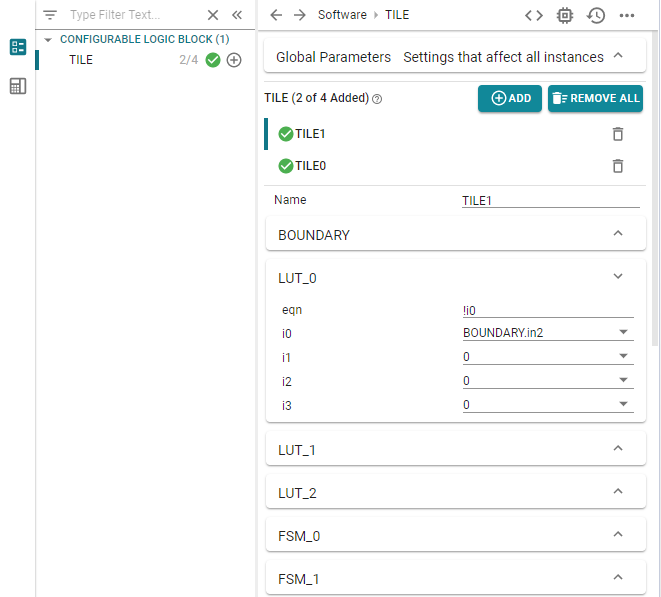
\includegraphics[width=8cm]{clbtool}}
    \caption{Grafično okolje ``CLB Tool''}
    \label{fig:clbtool} 
\end{figure} 

Grafični vmesnik za vsako od komponent, naštetih v poglavju
\ref{sec:zgradbaclb}, dovoljuje izbiro opisanih parametrov, vhodnih in izhodnih
signalov ter splošno konfiguracijo modulov. Kot je prikazano na sliki
\ref{fig:clbtool_struktura}, orodje generira 2 aplikacijski datoteki;
``clb\_config.h'' ter ``clb\_config.c''. Ti datoteki lahko seveda brez težav
vključimo v naš ``C'' program.

\begin{figure}[htb]
    \centerline{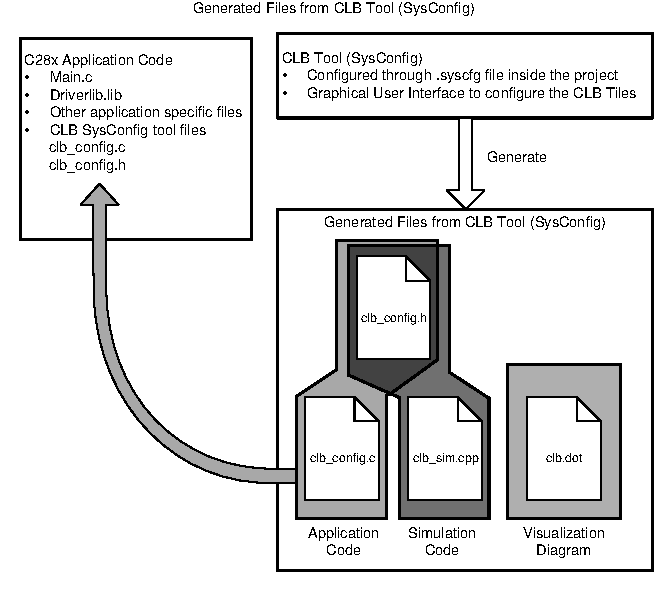
\includegraphics[width=8cm]{clbtool_struktura}}
    \caption{Struktura projekta pri uporabi orodja ``CLB Tool''
             \cite[Pogl.~1]{clb-user-guide}}
    \label{fig:clbtool_struktura} 
\end{figure} 

Poleg aplikacijske kode, pa nam orodje avtomatsko zgenerira tudi simulacijsko
datoteko ``CLB.vcd''. Gre za datoteko, v kateri je zapisan potek časovnih
signalov v koprocesorju. Odpremo jo lahko z zunanjim programom, ki omogoča
prikaz njene vsebine, s čimer posredno pridobimo vpogled v vse signale v
CLB-ju. Na primeru s slike \ref{fig:clbtool_simulacija} je v ta namen
uporabljen program ``GTK wave''.

\begin{figure}[htb]
    \centerline{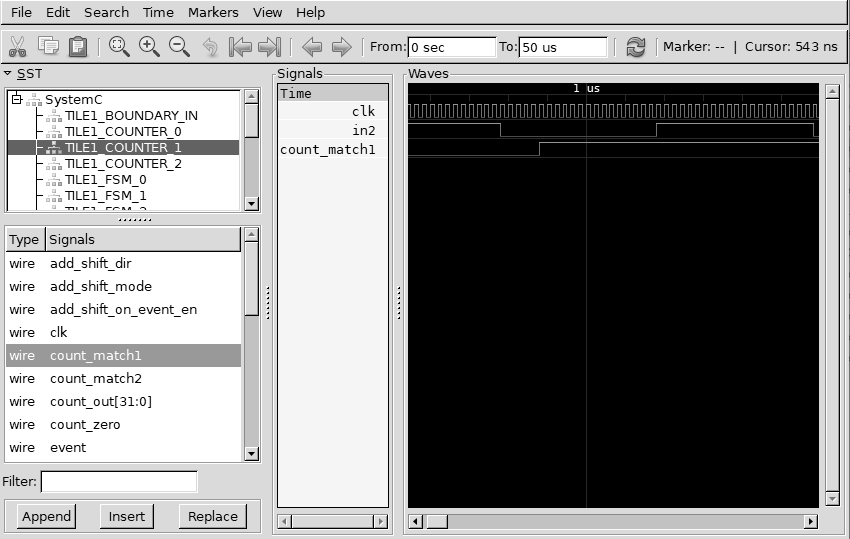
\includegraphics[width=8cm]{gtkwave}}
    \caption{Pregled notranjih signalov CLB-ja s programom ``GTK Wave''}
    \label{fig:clbtool_simulacija} 
\end{figure} 

Orodje avtomatsko generira tudi datoteko za grafični pregled povezav v
koprocesorju. Ta se prevede v obliko ``.html'', ki jo lahko odpremo v vsakem
brskalniku (slika \ref{fig:clbtool_diagram}) \cite[Pogl.~1]{clb-user-guide}.

\begin{figure}[htb]
    \centerline{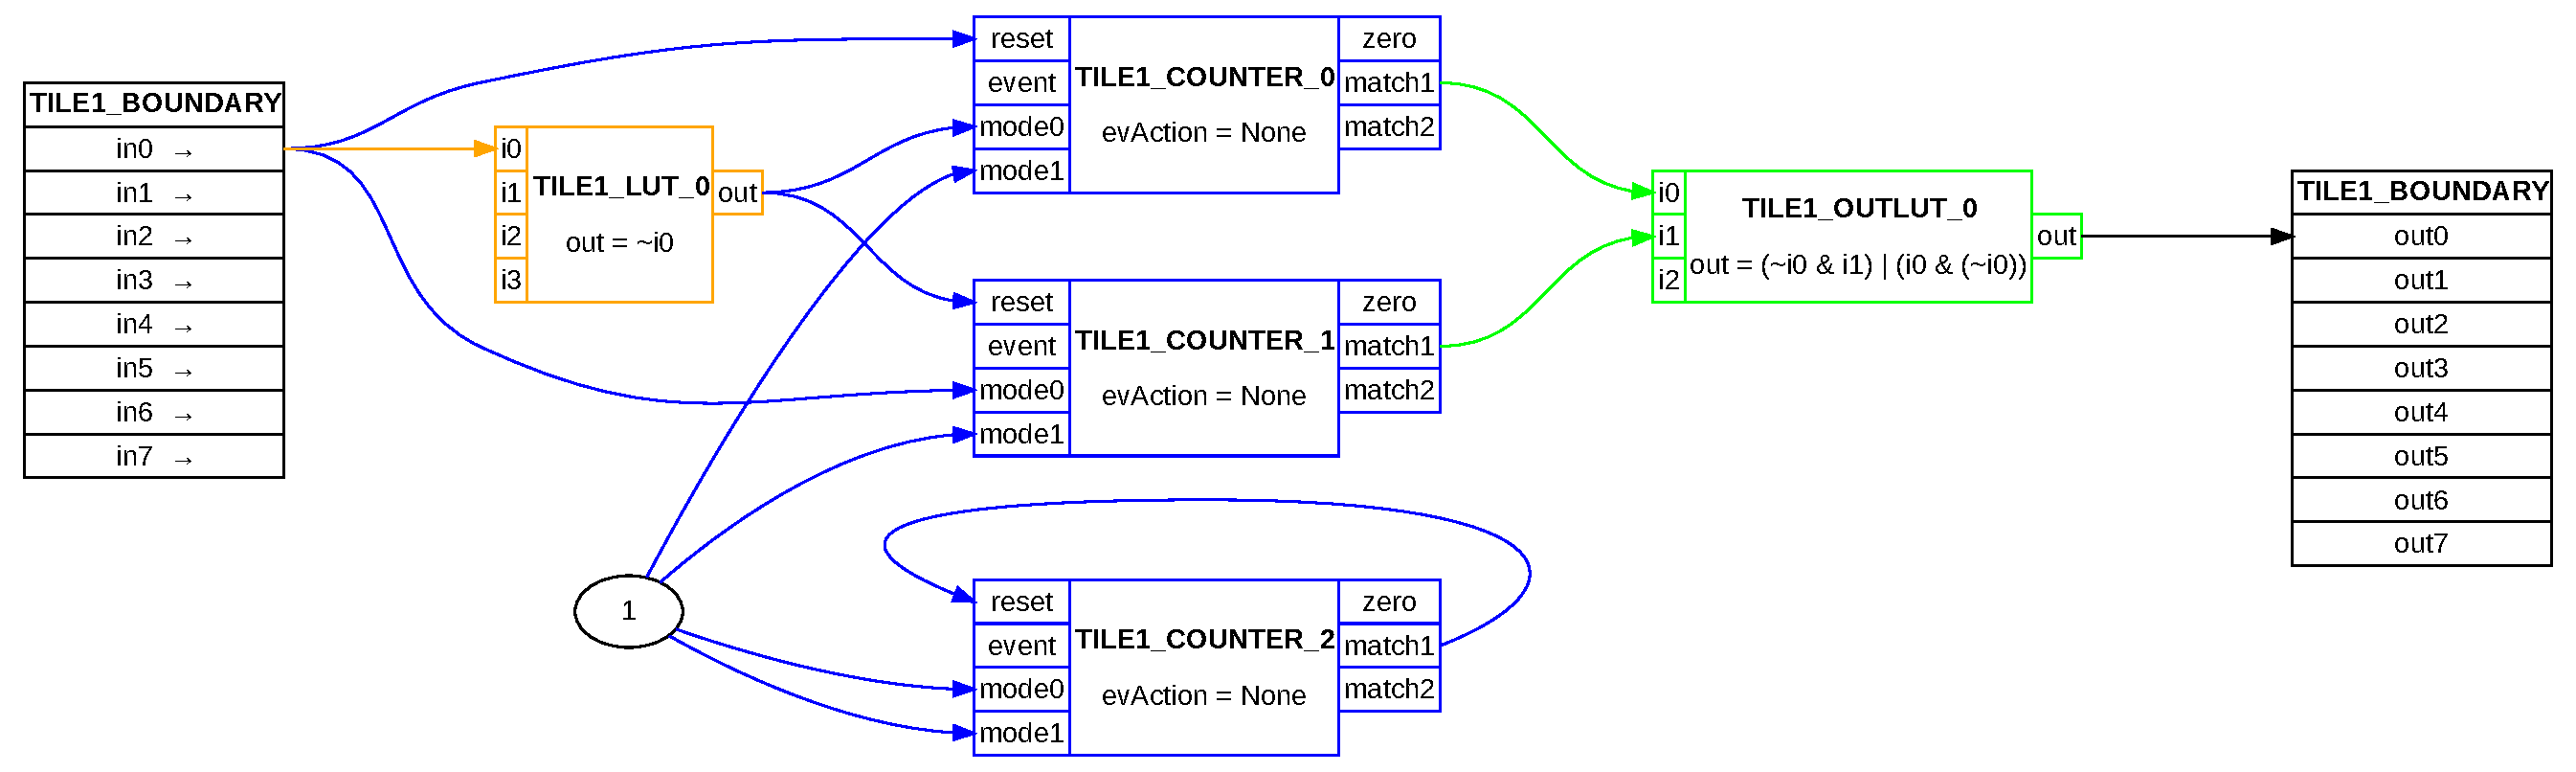
\includegraphics[width=8cm]{html_diagram}}
    \caption{Primer generiranega ``.html'' diagrama}
    \label{fig:clbtool_diagram} 
\end{figure} 


\section{Zaključek}
Za programerja FPGA vezij so stvari, opisane v tem članku verjetno precej
domače. Lahko pa opazimo da sam CLB ni le FPGA vdelan v mikrokrmilnik, vendar
prinaša tudi nekatere novosti (npr. HLC), zaradi katerih je marsikatera
aplikacija dokaj lažja za implementacijo.

Poleg tega so na voljo tudi precej močna tudi orodja v opisanem ekosistemu.
Grafično orodje omogoča uporabo tudi manj veščim programerjem. Dodatne
generirane simulacijske datoteke pa so v veliko situacijah nepogrešljive, saj s
samim opazovanjem zunanjih signalov težko odkrijemo morebitno napako. Enako
velja za generirani diagram, ki je (če že ne drugače) uporaben za odkrivanje
napačnih in nepotrebnih povezav med posameznimi moduli v koprocesorju.

Vendar pa tudi CLB, kot vsaka stvar ne pride brez pomankljivosti. Skoraj vsaka
``izboljšava'' nad FPGA s seboj prinese tudi kakšno frustracijo za programerja;
grafični vmesnih ``CLB Tool'' je na prvi pogled res prijazen, a se zaradi
velike abstrakcije kaj hitro izgubimo med neštetimi nastavitvenimi meniji.

Kljub temu pa lahko rečemo, da je takšna izvedba dodatnega modula zelo
smiselna. Nemalokrat se znajdemo v situaciji, kjer bi bilo potrebno modulirati
nek signal, vendar je samo zanj uporaba dodatnega čipa nesmiselna. Poleg tega
pa je s stališča delodajalcev velikokrat bolj smiselno uporabiti rešitev, ki jo
lahko implementira obstoječ kader, kot pa iskanje znanja izven podjetja.


\printbibliography


\end{sloppypar}
\end{document}
